\section{Exact multivariate amplitude distributions}
\label{sec:exact_distributions}


In Sect. \ref{subsec:general_considerations} we set the theoretical
considerations to construct the distributions. In Sect.
\ref{subsec:distributions} we define the four distribution cases and in Sect.
\ref{subsec:graphical_distributions} we show their graphical representation.

%%%%%%%%%%%%%%%%%%%%%%%%%%%%%%%%%%%%%%%%%%%%%%%%%%%%%%%%%%%%%%%%%%%%%%%%%%%%%%%
\subsection{General considerations}\label{subsec:general_considerations}

To compare the $K$ variate distributions with data, the crucial idea is to
construct $K$ univariate distributions out of the $K$ variate one which are
then overlaid \cite{exact_distributions_guhr}. To decouple the amplitudes, we
rotate the vector $r$ into the eigenbasis of the eigenbasis of the covariance
matrix $\Sigma$ \cite{non_stationarity_fin_guhr,exact_distributions_guhr}. More
precisely, we use the diagonalization
\begin{align}
    \Sigma = U \Lambda U^{\dagger} \text{ such that }
    \Sigma^{-1/2} = U \Lambda^{-1/2} U^{\dagger},
\end{align}
where $U$ is an orthogonal $K \times K$ matrix and $\Lambda$ is the diagonal
matrix of the eigenvalues $\Lambda_{k}$. As they are positive definite, the
square roots $\Lambda_{k}^{1/2}$ are real, so we choose them positive. We use
the rotated amplitudes
\begin{equation}
    \tilde{r} = U^{\dagger} r
\end{equation}
as new arguments of the ensemble averaged amplitude distribution.

When analyzing data, $K$ is given, we obtain the matrix $\Sigma$ by using the
originally measured amplitudes for sampling over the long time interval. In all
cases, the parameter N is a fit parameter, measuring the strength of the
fluctuations. Experience tells that $N$ sensitively determines the shape and is
best obtained by fitting the whole distribution to the data. For three cases,
the parameters $L$ and $l$ are shape parameters.

%%%%%%%%%%%%%%%%%%%%%%%%%%%%%%%%%%%%%%%%%%%%%%%%%%%%%%%%%%%%%%%%%%%%%%%%%%%%%%%
\subsection{Four cases distributions}\label{subsec:distributions}

As the aim of this paper is to compare the proposed distributions with
empirical data, we present the final form of the corresponding distributions.
For a detailed and complete explanation of the process to obtain the
distributions, we suggest reviewing the work of Guhr and Schell
\cite{exact_distributions_guhr}.

For the following cases, $K$ is the number of companies,
$\Gamma\left(\ldots\right)$ is the gamma function, $\Lambda_{k}$ is the $k$-th
eigenvalue of $\Sigma$, $\operatorname{K\left(\ldots\right)}$ is the modified
Bessel function of second kind, $\operatorname{U}\left(\ldots\right)$ is the
confluent hypergeometric function and
$_{2}\operatorname{F}_{1}\left(\ldots\right)$ is the Gauss hypergeometric
function. $N$ is a fit parameter, and $M$, $m$, $L$ and $l$ are shape
parameters. We use Eq. \ref{eq:m_relation} to compute $m$ and
\begin{equation}
    M = 2L - K - N - 1
\end{equation}
to compute $M$.

In the Gaussian-Gaussian case with the Markovian situation $D = \mathbb{1}_{N}$
the distribution reads
\begin{equation}
    \left\langle p \right\rangle_{GG}^{\left(k\right)}
    \left(\tilde{r}_{k} \vert \Lambda_{k}, \mathbb{1}_{N}\right) =
    \frac{1}{2^{\left(N - 1\right) / 2} \Gamma \left(N / 2\right)
    \sqrt{\pi \Lambda_{k} / N}}
    {\sqrt{\frac{N \tilde{r}_{k}^2}{\Lambda_{k}}}}^{\left(N - 1\right) / 2}
    \operatorname{K}_{\left(1 - N\right)/2}
    \left( \sqrt{\frac{N \tilde{r}^2_{k}}{\Lambda_{k}}}\right),
\end{equation}
In the Gaussian-algebraic case with the Markovian situation
$D = \mathbb{1}_{N}$ the distribution reads
\begin{equation}
    \begin{split}
    \left\langle p \right\rangle_{GA}^{\left(k\right)}
    \left(\tilde{r}_{k} \vert \Lambda_{k}, \mathbb{1}_{N}\right) =
    &\frac{\Gamma\left(L - \left(K + N \right) / 2 + 1\right)
    \Gamma\left(L - \left(K - 1\right) / 2\right)}
    {\Gamma\left(L - \left(K + N - 1\right) / 2\right) \Gamma\left(N / 2\right)
    \sqrt{2\pi \Lambda_{k}M/N}} \\
    & \operatorname{U} \left(L - \frac{K + N}{2} + 1, \frac{1 - N}{2} + 1,
    \frac{N}{2M} \frac{\tilde{r}^{2}_{k}}{\Lambda_{k}}\right)
    \end{split}
\end{equation}
In the algebraic-Gaussian case with the Markovian situation
$D = \mathbb{1}_{N}$ the distribution reads
\begin{equation}
    \begin{split}
    \left\langle p \right\rangle_{AG}^{\left(k\right)}
    \left(\tilde{r}_{k} \vert \Lambda_{k}, \mathbb{1}_{N}\right) =
    &\frac{\Gamma\left(l - \left(K - 1 \right) / 2\right)
    \Gamma\left(l - \left(K - N\right) / 2\right)}
    {\Gamma\left(l - K / 2\right) \Gamma\left(N / 2\right)
    \sqrt{2\pi \Lambda_{k}m/N}} \\
    & \operatorname{U} \left(l - \frac{K - 1}{2}, \frac{1 - N}{2} + 1,
    \frac{N}{2m} \frac{\tilde{r}^{2}_{k}}{\Lambda_{k}}\right)
    \end{split}
\end{equation}
Finally, in the algebraic-algebraic case with the Markovian situation
$D = \mathbb{1}_{N}$ the distribution reads
\begin{equation}
    \begin{split}
    \left\langle p \right\rangle_{AA}^{\left(k\right)}
    \left(\tilde{r}_{k} \vert \Lambda_{k}, \mathbb{1}_{N}\right) =
    &\frac{\Gamma\left(l - \left(K - 1 \right) / 2\right)
    \Gamma\left(l - \left(K - N\right) / 2\right)}
    {\Gamma\left(l - K/ 2\right) \Gamma\left(L + l - \left(K - 1\right) \right)
    \sqrt{\pi \Lambda_{k}Mm/N}} \\
    &\frac{\Gamma\left(L - \left(K + N \right) / 2 + 1\right)
    \Gamma\left(L - \left(K - 1\right) / 2\right)}
    {\Gamma\left(L - \left(K + N - 1\right) / 2\right) \Gamma\left(N / 2\right)
    } \\
    & _{2}\operatorname{F}_{1} \left(l - \frac{K - 1}{2}, L -\frac{K + N}{2}+1,
    L + l - \left(K - 1\right), 1 - \frac{N}{Mm} \frac{\tilde{r}^{2}_{k}}
    {\Lambda_{k}}\right).
    \end{split}
\end{equation}

For a visual comparison of the distributions, we plot the GG, GA, AG and AA
distributions in the Markovian case in the same figure. In Fig.
\ref{fig:distributions_comparison} we consider $K = 100$ positions with shape
parameters $L = 55$, $l = 55$, as well as $N = 5$ which is a typical value from
an empirical viewpoint. In the top are the probability densities in linear
scale and in the bottom are the probability densities in logarithmic scales.
From the figure, it can be seen that the more algebraic, the stronger peaked is
the distribution and heavier are the tails.

\begin{figure}[htbp]
    \centering
    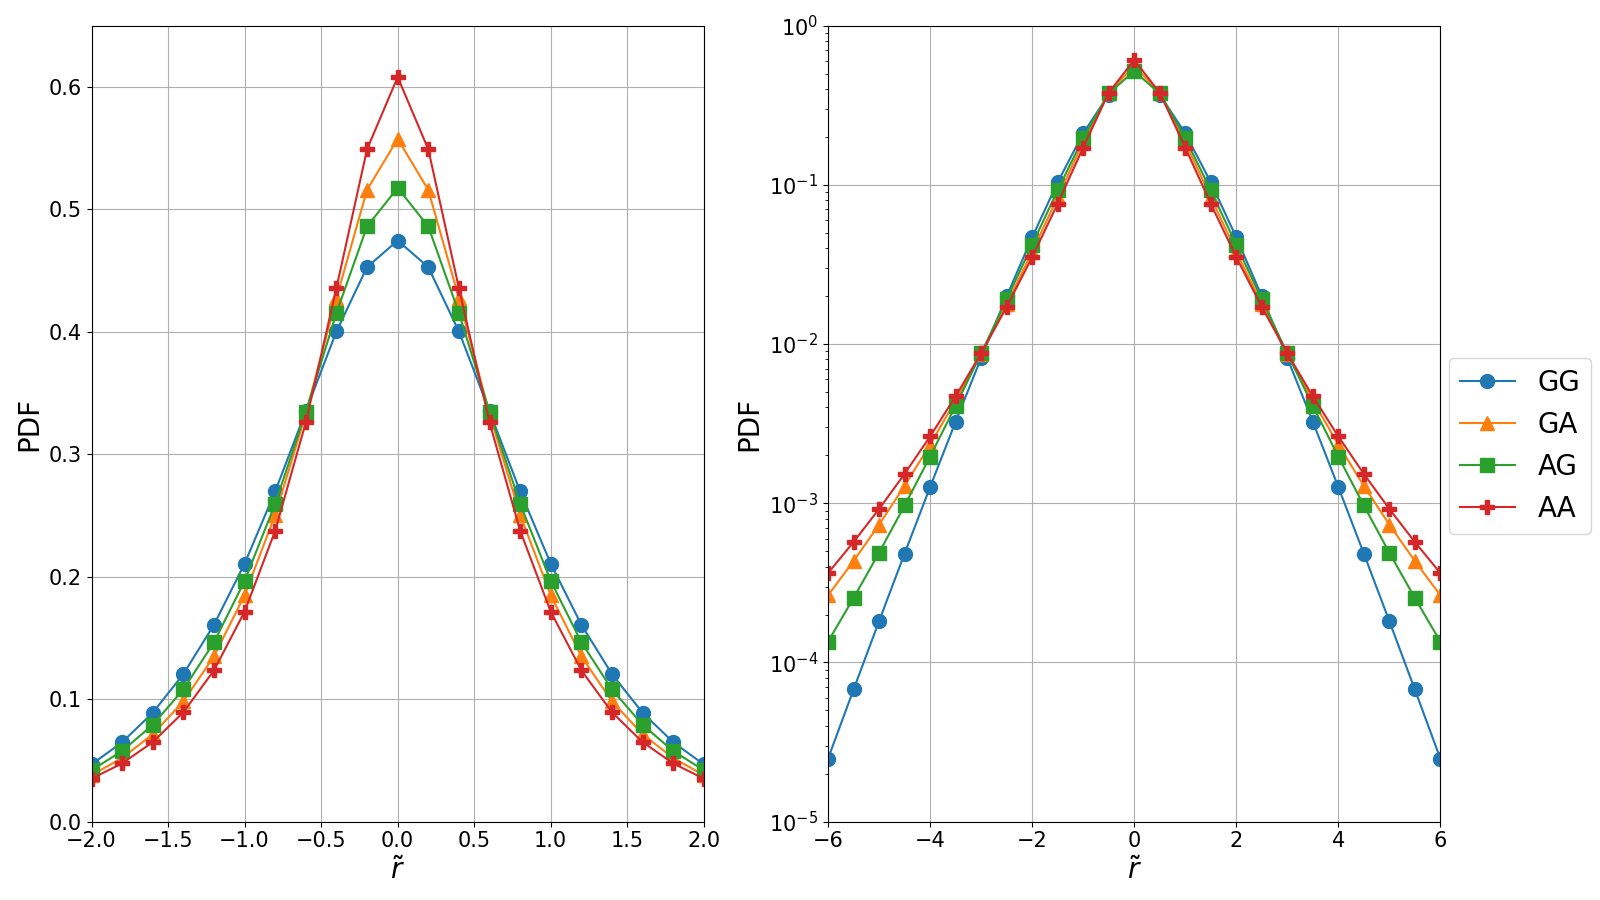
\includegraphics[width=0.9\columnwidth]
    {figures/07_distributions_comparison.png}
    \caption{Probability densities
             $\left\langle p \right\rangle_{YY'}^{\left(k\right)}$, in the
             Markovian case versus the rotated amplitudes $\tilde{r}$,
             normalized to unit standard deviation. The four cases
             Gaussian-Gaussian, Gaussian-Algebraic, Algebraic-Gaussian and
             Algebraic-Algebraic are labeled $YY' = GG$, $GA$, $AG$ and $AA$,
             respectively. Number of positions $K = 100$, shape parameters
             $L = 55$ and $l = 55$, strength parameter for fluctuations of
             correlations $N = 5$. (left) linear scale and (right) logarithmic
             scale.}
    \label{fig:distributions_comparison}
\end{figure}

%%%%%%%%%%%%%%%%%%%%%%%%%%%%%%%%%%%%%%%%%%%%%%%%%%%%%%%%%%%%%%%%%%%%%%%%%%%%%%%
\subsection{Graphical representations}\label{subsec:graphical_distributions}

To plot a comparison of the distributions involving algebraic distributions
with those in the Gaussian-Gaussian case, we choose values of $L$ and $l$ which
ensure the existence of the first matrix moment. We notice that the conditions
on the existence of the algebraic distributions, i.e., of their normalizations,
are slightly weaker. The variances
$\left\langle \tilde{r}_{k} \right\rangle_{YY'}{\left(k\right)}$ are simply
given by $\Lambda_{k}$. The functional form of all distributions
$\left\langle p \right\rangle_{YY'}{\left(k\right)} \left(\tilde{r}_{k} \vert D \right)$
then allows us to normalize the rotated amplitude $\tilde{r}_k$ by the standard
deviation
\begin{equation}
    \tilde{r} = \frac{\tilde{r}_{k}}{\sqrt{\Lambda_{k}}}
\end{equation}
such that all $K$ distributions in this variable coincide and the corresponding
variances are all given by one.